\documentclass[11pt,letterpaper]{article}
\usepackage{array}
\usepackage[in]{fullpage}
\usepackage{verbatim}
\usepackage{parskip}
\usepackage{graphicx}

\usepackage{titlesec}
\titlespacing{\section}{0pt}{\baselineskip}{0pt}
\titleformat*{\section}{\normalsize\bfseries\MakeUppercase}

\titlespacing{\subsection}{0pt}{0.5\baselineskip}{0pt}
\titleformat*{\subsection}{\normalsize\bfseries}

\titlespacing{\subsubsection}{0pt}{0.5\baselineskip}{0pt}
\titleformat*{\subsubsection}{\normalsize\bfseries}

%\setlength{\parindent}{0in}

\begin{document}
\setlength{\parindent}{0in}
%\baselineskip 4pt
\newcommand{\tablespace}[0]{\vspace{8pt}}
\textbf{ENVS S422: Earth's Climate System\\
Modeling Exercise 6: The rock cycle}\\%\footnote{Based on exercises developed by Dave Bice at Penn State University.}}\\

The rock cycle was probably the first of Earth's cycles or systems to be recognized and studied, at least qualitatively. It is presented in practically every introductory geology textbook as a sort of broad, all-encompassing framework for understanding the details of rocks and minerals --- the traditional bread and butter of geology. The processes involved in this cycle are generally well-known and thoroughly covered in textbooks, but very little work has been done on modeling the rates and behavior of the system as a whole. In this exercise you use will a simple model to explore the behavior of the rock cycle.

For each model experiment, you should submit a 1- to 2-paragraph response to the questions that are being explored in the exercise and \textit{at least} one graph to help justify your response. This modeling exercise involves several reservoirs and flows. I would like you to focus on explaining the relative timing and magnitude of the changes in the reservoir values.

Due date: 8 April 2019

\section{Introduction to the rock cycle}
\begin{figure}[h]
\center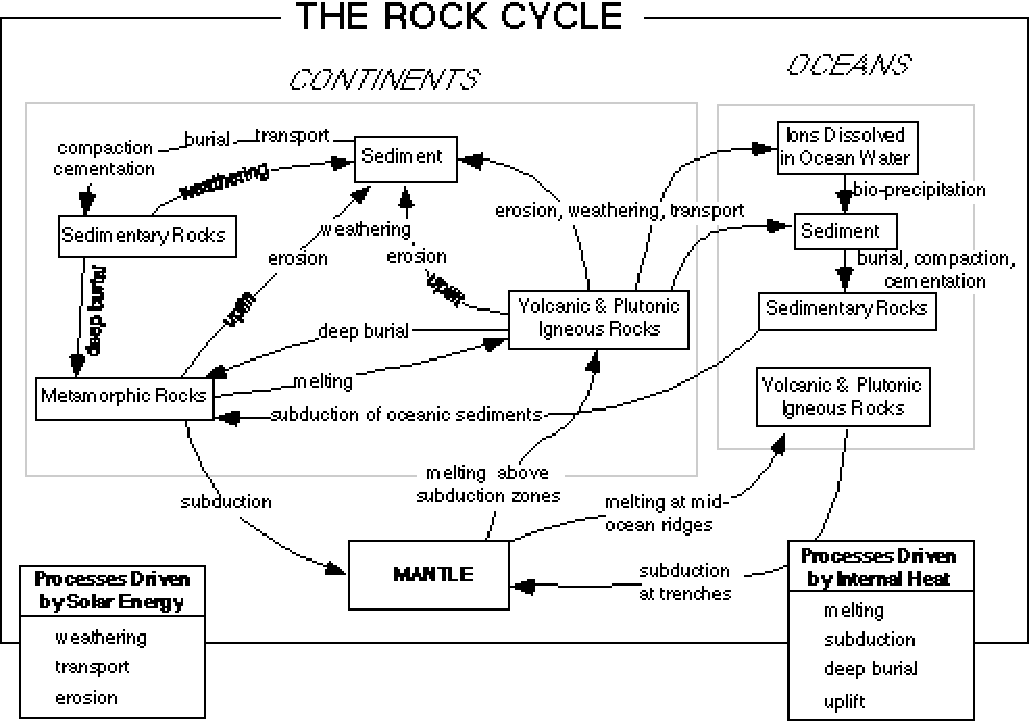
\includegraphics[width=4in]{./rock_cycle}
\end{figure}

In the figure above, the boxes represent different kinds of rocks and the arrows represent processes that not only transport materials from one reservoir to another, they also transform the rocks from one form to another. So for instance, one kilogram of granite, a plutonic igneous rock, is broken down by a variety of chemical and physical weathering processes when it is exposed at the Earth's surface; this kilogram of material then takes the form of sedimentary particles that commonly get transported away from the site of weathering to a final resting place where the are deposited and eventually form a kilogram of sedimentary rock. In reality, some of the starting kilogram is carried away in solution and ends up in the ocean where it will eventually be deposited, perhaps with the help of some organism, to form another kind of sedimentary rock. So, our starting kilogram of granite may end up getting dispersed to different places, but it will all end up forming a sedimentary rock --- conservation of mass applies to these processes of transformation if we consider them on a global scale. Another important point to understand is that the reservoirs do not really represent things that have well-defined boundaries like a tub of water; each reservoir represents a particular state or condition of rock-forming materials. This drawing above of the rock cycle is fairly complex, so it is worth going systematically and tracing out all the possible flow paths that rock-forming materials may follow.

It is also important to have a proper sense of time before starting in on this modeling exercise. In human terms, the rock cycle is incredibly sluggish --- we're talking about hundreds of millions of years. It is even slow in comparison to many of the surficial systems on Earth; this is why we still have a few rocks that are nearly 4 billion years old. There are also important spatial variations --- the interiors of large continents are not nearly as active as the edges of continents and the boundaries of plates. The changes within oceanic plates are even faster, as evidenced by the fact that we have virtually no pieces of intact oceanic crust older than 180 million years old.

What powers this system? The most important driving forces are (1) heat from the interior of the Earth, which causes plate tectonics to operate, leading to metamorphism, deep burial of rocks, melting of rocks, and rock uplift, and (2) solar energy, which powers the surficial processes of weathering and transport. We will initially assume that these driving forces are constant over time, but there are many reasons to believe that important variations occur; we will consider these variations in some of the later experiments.


%----------------------------------------------------------------------------------------
%----------------------------------------------------------------------------------------
\section{Model components}
\subsection{Reservoirs}
Our model will be somewhat simpler than the figure shown above; we will ignore the sediment deposited on oceanic crust, leaving us with just one sediment reservoir and one sedimentary rocks reservoir. Altogether, then, we will have 6 different reservoirs:
\begin{enumerate}
\item Mantle (the asthenosphere -- extending no deeper than 670 km below the surface)
\item Oceanic igneous rocks
\item Continental igneous rocks
\item Metamorphic rocks
\item Sedimentary rocks
\item Sediments (loose, unconsolidated particles, not yet rocks)
\end{enumerate}

In the model we will keep track of the mass of material in each reservoir. The
initial masses are provided in the table on the next page.
\begin{table}[h]
\begin{tabular}{lcccc}
Reservoir & \hspace{5pt} Volume (km$^3$) \hspace{5pt}& \hspace{5pt} Density (Pg/km$^3$) \hspace{5pt} & \hspace{5pt} Mass (Pg) \hspace{5pt} & \hspace{5pt} \% of Total \hspace{5pt}\\
\hline
Mantle & 2.97E+11 & 3.30 & 9.80E+11 & 97.42\\ 
Oceanic igneous rocks & 1.86E+09 & 2.90 & 5.39E+09 & 0.54\\
Continental igneous rocks & 4.92E+09 & 2.70 & 1.33E+10 & 1.32\\
Metamorphic rocks & 2.08E+09 & 2.70 & 5.62E+09 & 0.56\\
Sedimentary rocks & 6.00E+08 & 2.50 & 1.50E+09 & 0.15\\
Sediments & 6.00E+07 & 2.20 & 1.32E+08 & 0.01\\
\hline
TOTAL MASS & & & 1.01e+12 &\\
\hline 
\end{tabular}
\end{table}

Note: Pg stands for petagram; 1 Pg=10$^{15}$ g.


\subsection{Flow processes}
The next things to consider are the processes involved in this model. Altogether, there will be eleven processes in our model of the rock cycle; each process is briefly described in the following paragraphs.

\subsubsection{Ocean crust production}
New ocean crust is produced at mid-ocean ridges, where two plates diverge from each other. Here, in response to the divergent motions, mantle material rises up to fill the void and as it rises, part of it melts. This molten material, magma, erupts on the sea floor and cools in place below the seafloor to form new oceanic crust. The new crust adheres in equal amounts to each of the two plates --- this is the way that oceanic plates grow. The rocks formed by this process are basalts and gabbros. The rate of formation is a function of the length of mid-ocean ridges and the average rate of plate motions, both of which may change over time. Initially, we will set this process to be a constant rate, equal to the present day value; a sensitivity to plate tectonic variations will be added later.

\subsubsection{Ocean crust subduction}
Ocean crust is destroyed through the process of subduction --- the sinking of cold, dense slabs of oceanic plates along plate boundaries where plate converge on each other. The subducted oceanic crust undergoes metamorphism and partial melting as it descends; the molten material then rises to form volcanoes while the metamorphosed remnants eventually remix with the rest of the mantle. These plate boundaries are associated with deep, narrow trenches and they are clearly delineated in three dimensions by the locations of earthquakes, which occur within and along the edges of the subducting plates. In general, almost all of the oceanic crust gets subducted, with the exception of protruding seamounts, plateaus, and other irregularities. Most of the sediment lying on top of the oceanic crust is also carried down into the mantle, undergoing metamorphism on its way to partially melting at depths of around 100 to 300 km below the surface. Like the production of oceanic crust, the destruction is also dependent on things like the length of subduction zones (which are generally about equal to the length of mid-ocean ridges) and the average rate of plate motions. This process will be defined in the same manner as the ocean crust production.

\subsubsection{Arc volcanism}
As mentioned above, when subduction occurs, molten material is generated; this magma has a different composition than the materials it is derived from, leading to the formation of rocks like andesite and even granite --- the starting materials for continental crust. The magma rises up to the surface forming volcanoes like Mt. St. Helens that occur in a line or an arc, paralleling subduction zones, giving rise to the term volcanic arcs. Volcanic arcs occur where the subducting plate reaches depths between 100 and 300 km; this is where the temperatures and pressures necessary for melting occur. We can think of these volcanic arcs as the places where new continental crustal material is formed and it turns out that this is the principle mode of formation; many other processes rework and reshape this arc material, but we can still think of the volcanic arc as the primary source of continental crust. The rate of arc volcanism is largely controlled by the length of subduction zones; the rate of subduction seems not to matter much. This process will be defined in the same manner as the ocean crust production and subduction.

\subsubsection{Weathering of continental igneous rocks}
When continental igneous rocks are exposed at the surface, they suffer chemical corrosion and physical abuse that we collectively call weathering. These rocks, many of which form far below the surface, are exposed as a result of uplift and erosion, which strips away overlying rocks. The most significant uplift and erosion occurs where large mountains ranges form --- at places where two large continents collide with each other (the Alps and Himalayas are examples of this kind of mountain chain). Weathering breaks the rocks down into a variety of products --- some material is carried away in solution and eventually ends up in the oceans; some material is in the form of new minerals such as clays (which commonly result from the alteration of feldspars), and some of the material is in the form of small rock and mineral particles in which there has been no mineralogical alteration from the parent rock. The non-soluble weathering products are carried away from the site of weathering by winds and running water; once these are liberated from the parent rock, they effectively become sediment particles and enter a new reservoir in our model. As mentioned above, this rate is tied to mountain-building activities, but it is also tied to simply the amount of continental igneous rocks that exist at any one time. For instance, if there are no continental igneous rocks, there will certainly be very little weathering of them. Conversely, if they make up a huge portion of the crustal rocks, then the weathering of them will be quite high. So, this process has some similarities to a typical ``draining'' flow and that is how we will represent it in our initial model.

\subsubsection{Lithification}
When sediment particles finally come to rest and are buried, they begin a process called lithification that will eventually turn them into sedimentary rocks. This is generally a slow process and requires pressure (supplied by the weight of overlying sediments) and usually some form of cement to bind together the different particles that make up the sedimentary rock. Cementation of many limestones occurs just after the particles are deposited on the seafloor, but many other types of sediment are not really lithified until they are buried to depths of up to a kilometer or more. The rate of lithification can be expected to vary according to how much sediment there is, so this flow will also be represented as being dependent on the reservoir it drains.

\subsubsection{Weathering of sedimentary rocks}
After sedimentary rocks form, they may undergo metamorphism or remain as sedimentary rocks, near the surface, for a long time, or they may be exposed and subjected to weathering processes. Rocks like limestones and dolostones and evaporites readily undergo dissolution and their products are carried away in solution by streams, eventually returning to the oceans. Other sedimentary rocks like sandstones and shales weather into sediment particles (often the same ones used to make the original sedimentary rock) and these particles then undergo transport and are eventually deposited to form new sedimentary rocks. Like the weathering of continental igneous rocks, this weathering flow will be defined so as to make it dependent on the reservoir it drains; when there is more sedimentary rock, there will be more weathering products from sedimentary rocks.

\subsubsection{Metamorphism of sedimentary rocks}
When sedimentary rocks are buried to depths greater than about 5 to 10 km, they experience high enough pressures and temperatures to metamorphose into new rocks. Metamorphism is generally just a rearrangement of all the elements that make up the minerals found in a rock, in order to produce a new set of minerals that are closer to being in equilibrium at these elevated temperatures and pressures. This rearrangement occurs by slow, solid-state diffusion of atoms -- no melting is involved in this process. It happens that at these high temperatures and pressures, the rocks become weaker and any forces acting on the rocks will cause them to deform, and this deformation leads to the alignment of minerals. This alignment gives the rocks a fabric in the form of foliated, banded, or lineated textures. Deep burial is one way of obtaining the heat necessary for metamorphism; heat from magma is another important agent in metamorphism and since magma production on the continents is associated with volcanic arcs and subduction zones, a great deal of metamorphism also occurs near convergent plate boundaries. The rate of this process is probably related in part on plate tectonics to the extent that plate tectonics controls the rate of arc volcanism and the occurrence of continental collisions that force some rocks to be buried to great depths. But, this process is also sensitive to the amount of sedimentary rock that exists, so it too can be represented in part as a typical draining flow.

\subsubsection{Metamorphism of continental igneous rocks}
Sedimentary rocks are not the only kinds of rocks to undergo metamorphism. Volcanic rocks, like sedimentary rocks, form at or near the surface, and so they generally require burial to undergo metamorphism. Plutonic igneous rocks, like granite, also undergo metamorphism, but unlike other rocks, they generally experience little in the way of mineralogical changes since the minerals found in granites are relatively stable at high temperatures because they formed at fairly high temperatures. But, the later heating of a rock like granite will cause it to become weak and susceptible to deformation. The deformation leads to the formation of a metamorphic fabric like gneissic banding. As with the metamorphism of sedimentary rocks, this process is tied in part to plate tectonics, and in part to the amount of rock material in the form of continental igneous rock; to begin with, it will be defined as a standard draining process.

\subsubsection{Melting of metamorphic rocks}
Metamorphic rocks can either remain as metamorphic rocks, or they can follow one of three paths --- melting, uplift and weathering, or subduction. Melting is simply the result of continued heating and leads to the production of magma and thus new igneous rocks when the magma cools. This process, like many of the others, will be defined so that it is dependent on the size of the reservoir it drains; later, we will also make it dependent on the relative intensity or activity of plate tectonics. 

\subsubsection{Weathering of metamorphic rocks}
Just like igneous and sedimentary rocks, metamorphic rocks are commonly uplifted and exposed through erosion of overlying rocks, and then they are subjected to weathering. The products of this weathering are of course particles of sediment that then undergo transport and eventually are deposited to form sedimentary rocks. Similar to the other weathering flows, we will define this flow as a draining process --- dependent on the size of the metamorphic rock reservoir.

\subsubsection{Metamorphic rock subduction}
Any rocks that get caught up in the dynamics of a subduction zone may eventually get dragged down along with the subducting oceanic plate and as they get dragged down, they undergo metamorphism. Some sizeable fraction of these rocks probably end up getting taken all the way down into the mantle, where they slowly mix with the rest of the mantle. This process is about the only way that rocks formed on the continents get recycled with the mantle. Like many of the other processes in this model, this one is probably controlled in part by the length of subduction plate boundaries and the rate of plate motions, but in part on the abundance of metamorphic rocks that exist or are being formed --- if the continents (all lumped together) were very small, for instance, there would be little continental rock adjacent to convergent plate margins where they could be subducted, whereas if there is a lot of continental material, then there is likely to be more continental material being subducted. To begin with, we will define this as a typical draining flow, and later we'll add in a sensitivity to variations in plate tectonics.

\subsection{Putting the model together}
The model that I am providing you as a starting point is given in the figure below.

\begin{figure}[h]
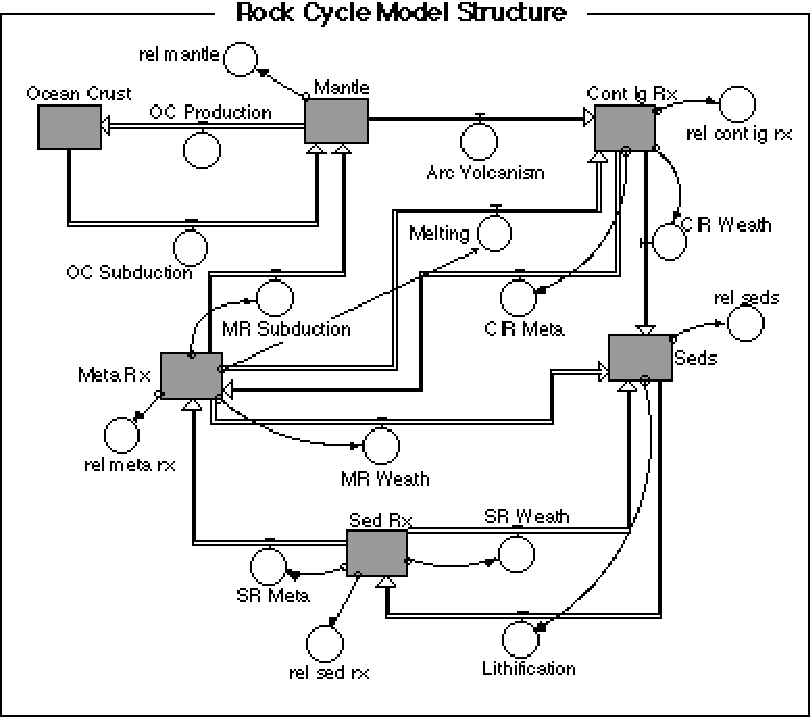
\includegraphics[width=3in]{./rcdiagram}
\end{figure}

Note that all of the flows except three have connector arrows indicating that they are dependent on the reservoir they flow out of. The three exceptions --- oceanic crust formation at mid-ocean ridges, oceanic crust subduction, and arc volcanism --- are flows that are principally controlled by plate tectonics. In other words, these flows are not a function of how much rock-forming material is in the mantle or any other reservoir; instead, they are controlled by forces that are external to this model.


\subsection{Flow values}
The actual magnitudes of most of these processes, in terms of mass transferred per time, can only be estimated. These estimates, summarized below, come from studying the modern environment and also from estimating the average age of different types of rocks. How does the average age provide useful information? In a simple system, the residence time is effectively the same as the average age of material within a reservoir, and the residence time is defined as:

\begin{verbatim}
residence time = amount in reservoir/total inputs or outputs
\end{verbatim}

This applies to the condition when the reservoir is in a steady state, in which case the sum of all the inputs must be the same as the sum of all the outputs. Thus, if we know the average age, we can approximate the residence time and in turn we can estimate the magnitudes of inflows and outflows. The table below shows the best estimates of some of the flows obtained from a study of the literature, along with the values recommended for use in the model. The values used in the model are defined such that they produce steady-state model solutions. For the model to be in a steady state, the amount of material in each reservoir must be constant over time, and for this to be the case, the inflows and outflows for each reservoir must be exactly equal to each other. Note that the time units have been altered quite a bit --- this will enable us to simulate the rock cycle for billions of years in a reasonable amount of time.

The sum of the three weathering flows, plus reworking of loose sediment, is estimated to be about 15 Pg/yr. With these basic data on initial reservoir amounts and steady state flow values, we
have all the information needed to construct the model. These data are assembled to
form the equations used in our starting model as shown below.

\begin{table}[h]
\begin{tabular}{lcc}
Flow & \hspace{5pt} Best Estimates (Pg/yr) \hspace{5pt}& \hspace{5pt} Model Value (Pg/100 Myr) \hspace{5pt}\\
\hline
Continetal crust production & 3.1--6.5 & 6.00E+08\\
Oceanic crust production & 50--75 & 7.00E+09\\
Oceanic crust subduction & 50--75 & 7.00E+09\\
Metamorphic rock subduction & $>$2 & 6.00E+08\\
Continental igneous rock weathering & * & 5.00E+08\\
Sedimentary rock weathering & * & 2.00E+08\\
Metamorphic rock weathering & * & 2.00E+08\\
Continental igneous rock metamorphism & no estimate in literature & 2.00E+08\\
Sedimentary rock metamorphism & 2--5 on continents & 7.00E+08\\
Metamorphic rock melting & no estimate in literature & 1.00E+08\\
Lithification & no estimate in literature & 9.00E+08\\
\hline 
\end{tabular}
\end{table}

\subsection{Model equations}
\subsubsection{Reservoirs}
\begin{verbatim}
INIT Mantle = 9.8E11 {Pg -- just asthenosphere}
INIT Ocean_Crust = 5.39E9 {Pg}
INIT Cont_Ig_Rx = 1.33E10 {Pg}
INIT Meta_Rx = 5.62E9 {Pg}
INIT Sed_Rx = 1.50E9 {Pg}
INIT Seds = 1.32E8 {Pg}
\end{verbatim}

\subsubsection{Flows}
\begin{verbatim}
OC_Production = 7.0E9 {Pg/100 Myr -- starting at today's rate}
OC_Subduction = 7.0E9 {Pg/100 Myr -- starting at today's rate}
Arc_Volcanism = 6E8 {units are Pg/100 Myr}
CIR_Weath = Cont_Ig_Rx*(5E8/1.33E10) {units are Pg/100 Myr}
CIR_Meta = Cont_Ig_Rx*(2E8/1.33E10) {units are Pg/100 Myr}
Lithification = Seds*(9E8/1.32E8) {units are Pg/100 Myr}
SR_Weath = Sed_Rx*(2E8/1.50E9) {units are Pg/100 Myr}
SR_Meta = Sed_Rx*(7E8/1.50E9) {units are Pg/100 Myr}
MR_Weath = Meta_Rx*(2E8/5.62E9) {units are Pg/100 Myr}
Melting = Meta_Rx*(1E8/5.62E9) {units are Pg/100 Myr}
MR_Subduction = Meta_Rx*(6E8/5.62E9) {units are Pg/100 Myr}
\end{verbatim}

\subsubsection{Converters}
\begin{verbatim}
rel_cont_ig_rx = Cont_Ig_Rx/1.33E10
rel_mantle = Mantle/9.8E11
rel_meta_rx = Meta_Rx/5.62E9
rel_seds = Seds/1.32E8
rel_sed_rx = Sed_Rx/1.50E9
\end{verbatim}

The converters at the end of this list of equations are devices that will be useful in monitoring the response of the model in some of the experiments outlined below --- they will enable us to plot all of the reservoirs with the same, normalized scale on the vertical axis. However, it may still be useful at times to plot each reservoir at a different scale so as to show the full range of change that each reservoir experiences.

At this point, we have everything necessary to create a fully-functional rock cycle model that is in a steady state (the model is provided to you). This steady-state model will be the control for the experiments. Test the model by running it for 1 billion years (10 of our time units since our flow rates are in units of Pg/100 Myr) with a time step of 0.1, using the Euler method of integration; also enter 100 Myr as the basic time unit. Graph some of the reservoir values to make sure that they are constant. 

\section{Experimenting with the rock cycle}
\subsection{Response time of the system}
The first set of experiments looks at how the system responds to changes; a major part of this question involves the length of time it takes for the system to respond to changes. As a first step, it will be helpful to go through and calculate the residence times or the apparent response times of each reservoir -- make a table showing the residence times for reservoirs with constant outflows and the response times for those reservoirs with draining outflows. I say ``apparent'' response time since none of these reservoirs really exists by itself and some of the flow processes are constants rather than normal draining flows. Nevertheless, this exercise will help us understand the overall behavior of the system. In a simple system --- one reservoir, one inflow, one outflow --- the response time is given by

\begin{verbatim}
response time = amount in reservoir / outflow
\end{verbatim}

For reservoirs without draining-type flows, where the flow values are constants, it is meaningless to talk about the response time, but instead, we can talk about another concept, the residence time, which is defined as

\begin{verbatim}
residence time = amount in reservoir / outflow (or inflow) at steady state
\end{verbatim}

You can see that for reservoirs with draining-type flows, the residence time and the response time are identical.

Now you are ready to do some experiments. The goal here is to investigate two different kinds of changes. First you will alter the initial value of one of the reservoirs and then you will alter the steady-state flow value that goes into defining one of the outflow equations. You will initially ``pick on'' the continental igneous rock reservoir since it is one of the biggest.
\bigskip

a) Change the initial amount in the Continental Igneous Rocks reservoir by multiplying the initial amount by 1.5, creating a 50\% increase in the starting value. To compensate for the mass increase in this reservoir, we will subtract the same mount from the Mantle reservoir. To do this, you could rewrite the Mantle initial value to the following:

\begin{verbatim}
INIT Mantle = 9.8E11 - 0.5*1.33E10
\end{verbatim}

What in the real world could cause this type of a change? A pulse of arc volcanism, for instance, would send a pulse of material into the Continental Igneous Rocks reservoir which would be similar to the instantaneous change we used in this experiment. Globally, arc volcanism is not likely to undergo such a pulse, but there have been episodes of brief, voluminous volcanic eruptions on the continents not related to arcs --- these are represented by flood basalt provinces, such as the one covering much of eastern Washington. Though these are not strictly related to arc volcanism, they do transfer material from the mantle to the reservoir of Continental Igneous Rocks, so it is reasonable to include them into the arc volcanism flow.

Run this model for a period of time equal to 5 billion years (50 time units) with a time step of 0.1 and the Euler method of integration. Before running the model, think carefully about what you expect to happen. Will all of the reservoirs be affected by this change? Will the system return to a steady state? If so, will that steady state be the same as the original, control or different? What are your reasons for making this prediction? What will be the response time of the whole system and how will the ``apparent'' response time of the separate reservoirs differ from their behavior in this connected model? You may find it useful to graph both the reservoir amounts and the relative amounts of each reservoir.
\bigskip

b) First, undo the change from the previous experiment, then change the steady state flow value used to define the weathering flow that transfers material from the Continental Igneous Rocks reservoir to the Sediment reservoir. To do this, rewrite the flow equation to:

\begin{verbatim}
CIR_weathering = Cont_Ig_Rx*(7.5E11/1.33E10)
\end{verbatim}

In so doing, we will increase the value of this flow by 50\% to begin with (because we changed 5E8 to 7.5E8, an increase of 50\%) -- this is the same amount of increase to this flow caused by initially increasing the amount in the Continental Igneous Rock reservoir, in the previous experiment. What in the real world could cause this type of a change? This kind of a change basically represents a change (an increase) in the nature of the process of weathering. This could be related to something like a climate change, making the average global climate warmer. Alternatively, it could represent some change in the biosphere; for example, with the rise of angiosperms (flowering plants), it is thought that the resulting increase in CO$_2$ in the soil would accelerate rates of weathering. The origin of land plants, which would have caused the first big jump in soil acids and CO$_2$, is another important occurrence that might be represented by this experiment.

The main question here is whether the system will behave in the same manner or not. If not, how will it differ and why? Give these questions careful thought in coming up with a prediction. (Remember to undo the changes you made for the previous experiment.) Then run the model for the same length of time and study the results to see how good your prediction was. If your prediction was off, take some time to figure out where you went wrong in your prediction.
\bigskip 

c) Test your understanding of this system. Do you understand what is going on when you make the two changes described above (experiments a and b)? If so, then you ought to be able to predict what will happen (in a general sense, not a precise, quantitative sense) if you apply these changes to another reservoir and its outflow. Try it out. If you are successful, you've made some real progress. If not, explore the model in more detail until you begin to see why your prediction was wrong. This may require that you do additional experiments. When doing so, remember to undo the
changes you made in previous experiments.

\subsection{Simulate the formation of the Earth}
This is not as hard as you might think. Start with your original, steady-state model, then estimate amounts for various reservoirs --- amounts that you feel represent likely conditions at the time when the Earth formed. Here, it may help to understand a bit about the early history of Earth, as far as we know (the lack of many rocks older than 3 to 4 billion years old presents a limit to how much we can say about this early history).

The Earth was formed around 4.6 billion years ago when particles left over from a violent supernova (a huge stellar explosion) accreted together, drawn by the gravitational force of our growing planet. These particles ranged in size from dust to huge masses perhaps even as large as Mars! In fact, the Moon is thought to have been produced from the remnants of a collision between a Mars-sized body and the early Earth. As the Earth grew, its gravitational attraction also grew and it attracted larger and larger particles, which, when they hit, released a tremendous amount of heat. All of this heat should have been sufficient to melt a good portion of the exterior of the Earth, creating an ocean of molten magma (imagine!). Eventually, as most of the debris in the solar system was swept up by planets, the impacts died down and so the early magma ocean would have been able to solidify, but there would always be a cooler, more brittle outer skin (the equivalent of plates today). All of this heating and bombardment would have released the gaseous components of the accreting material; some of these gases would be bound to the Earth by gravity, forming the early atmosphere and ocean. So, at the very beginning, once the magma ocean cooled, there was probably no real continental igneous rock, and thus no sediment or sedimentary rock or metamorphic rock; instead, the surface was covered with material similar to oceanic igneous rocks. 

With the above information, you are ready to proceed with this experiment. We will keep this experiment simple by assuming that the basic processes have not changed, meaning that we will not make any changes to the equations that define the flows. Instead, we will alter the initial amounts of the reservoirs, keeping the total mass the same. This will mean redistributing the material currently found in the continental reservoirs (including continental igneous rocks, sediments, sedimentary rocks, and metamorphic rocks) into the oceanic igneous rock and mantle reservoirs. It turns out not to matter much how you redistribute the material since none of the outflows from these two reservoir change. But, if you increase the oceanic igneous rock reservoir until it is 30\% larger, that would be equivalent to oceanic crust covering the whole planet. Then, you could take the remainder of the continental reservoirs and add that to the mantle. 

As always, make some predictions about what will happen. How long will it take for the system to evolve into a steady state? How will the resulting steady state compare with the present condition of the rock cycle (represented by the original control version of this model)? How will the model compare after 4.6 billion years of simulation time (46 time units) with the present Earth? After giving these questions some thought, run the model (again using a time step of 0.1) and see what happens. You may want to run it for 4.6 billion years first, and then run it for as long as it takes to arrive at a near steady state. If you find that after 4.6 billion years, the model does not arrive at the presently-observed condition of the real Earth, come up with some hypotheses to explain the discrepancy.

\subsection{Effects of tectonic variations}
In this experiment, we will investigate the effects of variations in tectonic activities. To do this, we will have to modify the model so that the appropriate flows are in some ways sensitive to the relative level of tectonic activity. Before doing this, we need to consider the natural variations in tectonic activity that have occurred over the course of Earth history. 

The key principle is that tectonic activity is primarily driven by heat and when heat is being released more rapidly, tectonic activity is expected to be more intense. Another key principle is that under normal circumstances, the rate of heat released by some body is directly proportional to the temperature gradient -- the change in temperature over distance. Since the majority of the heat within the Earth is residual heat from the energy of formation, the Earth has been cooling over time, although the cooling is slowed somewhat because of some heat produced by radioactive decay. This means that early on, the temperature at the very center was considerably higher, and since the surface temperature was probably not much different, the temperature gradient must have been higher -- thus the heat release must also have been greater than at present. It is estimated that in the beginning, the heat released was 2 to 3 times the present release, and this value has decreased exponentially over time. One of the main ways that heat is transferred from the interior to the surface is by convection (this process is nicely seen in a bowl of miso soup as the fluid rises, spreads across the surface, descends, and then rises again as a result of density changes that accompany temperature changes) and it appears that convection is not so uniform over time. Some of the variations may occur on a cycle that has a period of around 400 to 500 Myr (related to the super-continent cycle) while other variations may occur with less regularity. It appears that every now and then (the most recent one occurred around 100 Myr ago), a great deal of material accumulates at the base of the mantle and then rises up to the surface rather quickly, bringing a great deal of heat with it, leading to increased volcanic activity (this also happened to coincide with a time of rapid plate motions). So, there is both a long-term, exponential decline in heat release and shorter-term oscillations, and these changes in heat release are expected to cause changes in tectonic activity. We will conduct two experiments here; one that incorporates the long-term variation and another that incorporates on the short-term variations.
\bigskip

a) Long-Term Variations in Tectonic Activity.
Here, we investigate the effect of imposing a higher level of tectonic activity early in Earth's history on the overall evolution of the rock cycle. This experiment will effectively be a variation of experiment 2 above, where we started with no material in any of the continental reservoirs, and the results from experiment 2 will provide the control for this experiment. How can we modify the model to carry out this experiment? Since the precise connection between heat flow and tectonic activity is not well-understood, we will introduce into our model a graph that depicts changes in tectonic activity over time, with the understanding that heat flow is the underlying cause of this tectonic variation. To do this, create a new connector, label it ``tectonic activity'' double-click on it and set it equal to time, then click on the become graph button and make the graph similar to the one shown below.

\begin{figure}
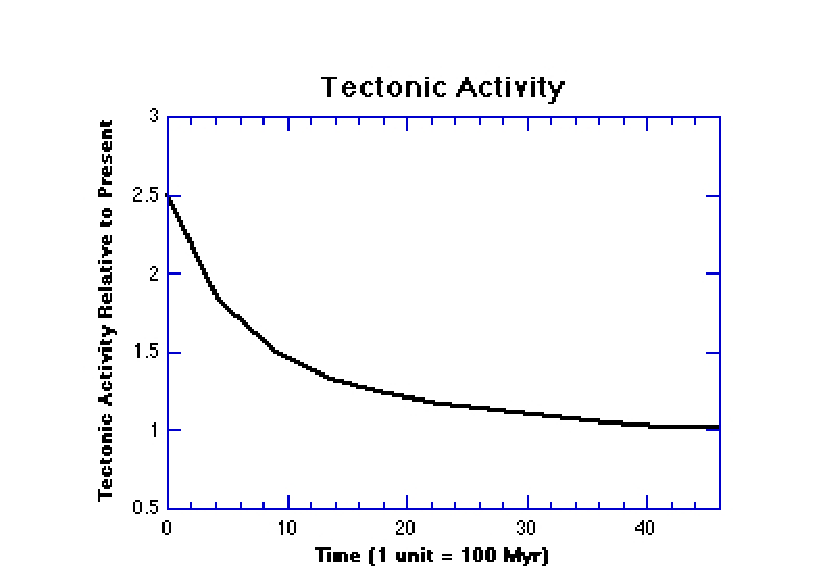
\includegraphics[width=3in]{./tectonic_activity}
\end{figure}

This will represent our first scenario in which we investigate the effects of just the long-term variation in tectonic activity due to the cooling of the Earth (note that this is roughly an exponential curve). The next step is to connect this tectonic activity converter to the appropriate flows. There are probably many ways that this could be done, but a simple approach will be to treat this tectonic activity value as a multiplier. This means making connecting arrows from tectonic activity to the appropriate flows and then multiplying that flow value (whether it is a constant or an equation) by tectonic activity. As mentioned in the discussion of processes above, the flows that are most likely to vary with tectonic activity are all of the metamorphism flows, melting, arc volcanism, and the production and subduction of oceanic crust.

Once you have made these changes and additions to the model, you are ready to run it, but before doing so, try to predict how this model will compare with the one you ran in experiment 2 above. As before, run this model for 4.6 billion years and compare the results with the present state of the rock cycle. You may find it useful to plot the tectonic activity converter along with the other model parameters. Study the control (results of experiment 2) in order to summarize the effect of the variations in tectonic activity.
\bigskip 

b) Short-Term Variations in Tectonic Activity.
Here, we will look into the effects of variations in tectonic activity that are equivalent to those associated with the supercontinent cycle (i.e., variations on the order of 400 to 500 Myr). To simplify this experiment, we will not superimpose this variation on the exponentially decreasing activity that we explored in the last model (although this could be an interesting experiment). For this experiment, we will modify the original version of the model --- the one with the initial values of the reservoirs set at their present-day levels. Redefine the tectonic activity converter to
\begin{verbatim}
tectonic activity = 1+SINWAVE(.5,5)
\end{verbatim}

This creates a sinusoidal variation from 0.5 to 1.5 with a period of 5 time units, which is 500 Myr. As above, we will use this converter as a multiplier, acting on the same flows that were modified in the above experiment (all of the metamorphism flows, melting, arc volcanism, and the production and subduction of oceanic crust.) In making your predictions about how the model will perform, think about which of the reservoirs are likely to change the most and which the least. Also, try to determine how the variations of the reservoirs will match up with the variations in tectonic activity --- when will each reservoir peak relative to the peaks in tectonic activity? Again, you will want to plot the tectonic activity converter along with the reservoirs in order to answer some of these questions. Run the model for 4.6 Byr with a time step of 0.1. You may find it difficult to see what is going on in the graphs resulting from this experiment if you plot 5 parameters in a single graph. One way to get around this is to go in and modify the vertical scales of the different parameters in order to separate them.
\end{document}
